% !TEX root = ../thesis.tex
\chapter{Lit Review}
	\label{chap:lit_review}
	
	
	\section{What is Comparative Judgement}
		Comparative judgement is a mathematical way to determine which observation item is better than the other item also being observed compared to each other. This method first got proposed in 1927 by Louis Leon Thurstone, a psychologist, under the term "the law of comparative judgement" \cite{thurstone1927psychophysical, thurstone1927law}. While comparative judgement is a technique that has been around for almost 100 years, it wasn't until the early nineties that this technique got proposed for use within an educational setting. This first proposal was by Politt and Murry \cite{pollitt1996raters}, who conducted a study where they tested candidates on their English proficiency within Cambridge's CPE speaking exam. The judges watched 2-minute videos and judged which one out of a pair of videos they deemed better at the requested task in the exam. However, before this, in the ninety seventies and eighties, comparative judgement was presented as a more theoretical basis for educational assessments \cite{andrich1978rating}. 
		
		With the momentum of his findings, Politt then presented comparative judgement as a tool for exam boards to use to be able to compare the standards of A-Levels from the different exam boards, replacing the direct judgement of a script that was at the time currently being used \cite{newton2007paired}. In his papers titled, "Let's Stop Marking Exams" \cite{stop_marking_pollitt}, he presents a valid argument for using comparative judgement, with the advantages it brings over some traditional types of marking.
		
		How comparative judgement works is to present two options to a marker. The marker then gets asked to pick which one of the two options they think is the better one. The marker will get presented with all possible combinations available, each time picking which one they think is the better one out of the two. An outputted score is then presented based on the method used. The original method, the Law of Comparative Judgement (LCJ), follows the formula:
		
		\begin{figure}[h]
			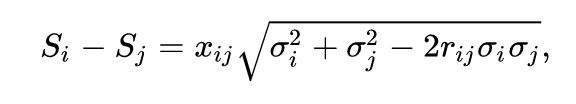
\includegraphics[width=8cm]{graphics/LCJ_formula.png}
			\caption{}
			\centering
		\end{figure}
	
		 $S_{i}$ is the psychological scale value of stimuli $i$
		%{\displaystyle x_{ij}} is the sigma corresponding with the proportion of occasions on which the magnitude of stimulus i is judged to exceed the magnitude of stimulus j
		%{\displaystyle \sigma _{i}} is the discriminal dispersion of a stimulus {\displaystyle R_{i}}
		%{\displaystyle r_{ij}} is the correlation between the discriminal deviations of stimuli i and j
		%The discriminal dispersion of a stimulus i is the dispersion of fluctuations of the discriminal process for a uniform repeated stimulus, denoted {\displaystyle R_{i}}, where {\displaystyle S_{i}} represents the mode of such values. Thurstone (1959, p. 20) used the term discriminal process to refer to the "psychological values of psychophysics"; that is, the values on a psychological continuum associated with a given stimulus.
		
		However, an alternative version derived from Louis Leon Thurstone, referred to as the "Pairwise Comparison" \cite{thurstone1927law}, will provide an output based on the difference between the quality values is equal to the log of the odds in respect to object-A will be object-B. This formula gets represented as: 
		$\displaystyle \mathrm {log\;odds} (A\ {\text{beats}}\ B\mid v_{a},v_{b})=v_{a}-v_{b} $.
		
		$\Pr\{X_{ji}=1\}={\frac {e^{{\delta _{j}}-{\delta _{i}}}}{1+e^{{\delta _{j}}-{\delta _{i}}}}}=\sigma (\delta _{j}-\delta _{i})$
		
		 .
		%\displaystyle \mathrm {log\;odds} (A\ {\text{beats}}\ B\mid v_{a},v_{b})=v_{a}-v_{b}}		


	\section{Tunnel your internet connection via the university internet}


	\section{Practice your Google Fu}
		\label{sec:google_fu}

%The internet is big \cite{sizeofinternet}.
%Knowing how to phrase a question to a search engine is therefore an invaluable skill.
If the request is simple enough, even a poorly structured query will likely return usable results.
For more difficult to find resources you can leverage the language of the search engine to gather relevant papers and resources for your research more efficiently. 
		
		% An example of how to centre a passage of text, control local font size, 
		% and create a properly formatted and clickable URL.
		\begin{center}
		{\small \url{https://www.gwern.net/Search}}
		\end{center}
		
``Internet Search Tips'' \cite{gwern} provides an excellent review of methods and tips for scouring the internet for hard to find resources.
You will also be less likely to get caught behind journal paywalls when working remotely without a tunnel as your queries can be made to look for raw PDFs that are often released by the authors directly.


	\section{Organising your citations in Bib\TeX{}}
		\label{sec:resources_bibtex}
	
Bib\TeX{} is a language for specifying resource citations.
Every time you access and read an academic paper, take code from an online repository, or source the media such as images from existing works, you should create a Bib\TeX{} entry in a file that you keep throughout your research.
Software such as Mendeley \cite{mendeley} can help automate the process of building your Bib\TeX{} library of citations. 
		
		\lstinputlisting[label={lst:bibtex}, caption={An example Bib\TeX{} entry for an academic paper published in conference proceedings \cite{kaj86}.}]{./listings/example_bibtex.bib}
		
The Bib\TeX{} code listing above (\cref{lst:bibtex}) shows an example of how to cite an academic paper; in this case one of the central papers in Computer Graphics research.
The key \textbf{kaj86} is an arbitrary name chosen as a meaningful identifier for the resource.
In the document text we can call on this resource as an inline citation using the \LaTeX{} command \lstinline|\cite{kaj86}|, which produces \cite{kaj86} at the location it is called.
As long as a citation has been used at least once somewhere within the document then a formatted full citation will be created in the bibliography at the end of the document with the same citation number that is shown inline.
		
It is considerably easier to be disciplined in methodically taking note of the resources you access and make use of as you access them than it is to try and hunt them all down again at the time you need to write about them in your document.
Invest time in being organised and consistent upfront and it will be easier when you come to write up.


	\section{Properly using and formatting citations within the text}

Usually you would not put the URL of the resource you are citing directly in the text like is done previously in \cref{sec:google_fu}.
The citation for the resource \cite{gwern} is sufficient to reference it within the text given that full details of its location are then kept neatly within the bibliography at the end of the document.

In normal usage the purpose of a citation is not to direct the reader away from your thesis, but to justify and back up assertions you are making about the state of the domain.
If a reader questions your assertions then they can follow the rabbit hole of papers which will likely also make and justify assertions with even earlier papers from the literature. 

In the above case the intention is for the reader of this template to actually go to that resource and read what it has to say directly.
The link is therefore shown clearly within the main text to indicate that the reader should visit it.
This as opposed to wanting the reader to purely acknowledge that the facts which are within the resource legitimise the points made in this document, in which case a simple inline citation is the best way to back up your assertions.
\Cref{sec:typesetting_figures_citation} specifically touches on the best practice for how to cite images which you are importing from existing work. 
